%Kelompok BSD
%Arjun Yuda Firwanda
%Dwi Septiani Tsaniyah
%Dwi Yulianingsih
%Ervanda Rambu Anarky
%Jeremia Wahyudi Sianturi

\section{Cara Mengkoneksi Sensor Pir}

Sensor Pir adalah sensor yang memiliki infrared yang memancar pada sensor yang mendeteksi adanya gerakan tangan.
Dengan demikian sensor pir bekerja pada sebuah gerakan dan infrared akan menangkap sinar dari sebuah gerakan yang akan mendeteksi si sensor pirnya dan dengan codingan yang benar angka akan mucul pada serial monitor.
Dalam melakukan percobaan sebuah sensor pir hendaknya mengetahui terlebih dahulu apa saja yang diperlukan dan bagaimana codingan yang benar untuk mengetahui sebuah sensor itu bergerak atau terdeteksi.

\subsection {Cara Merakit Sensor Pir dan Arduino}

Sebelum merakit sensor pir dan arduiono berikut yang perlu dilakukan sebelum merakit.
\begin{enumerate}
\item Pastikan kita mengetahui komponen sensor pir.
\item Mengetahui fungsi dan cara kerja sensor pir.
\end{enumerate}

\subsubsection {Tutorial Merakit Sensor Pir}
Alat yang diperlukan:
\begin{enumerate}
\item Arduino Uno.
\item Sensor Pir.
\item Lampu Led (warna bebas).
\item Kabel Jumper Male to Female (3 buah warna).
\item Kabel USB.
\item PC.
\end{enumerate}

Cara Merakit:
a. Gabungkan kabel jumper male to female berwarna orange dari VCC sensor pir ke pin 5 arduino seperti terlihat pada gambar \ref{carakoneksikabelvcc}.



\begin{figure} [ht]
\centerline{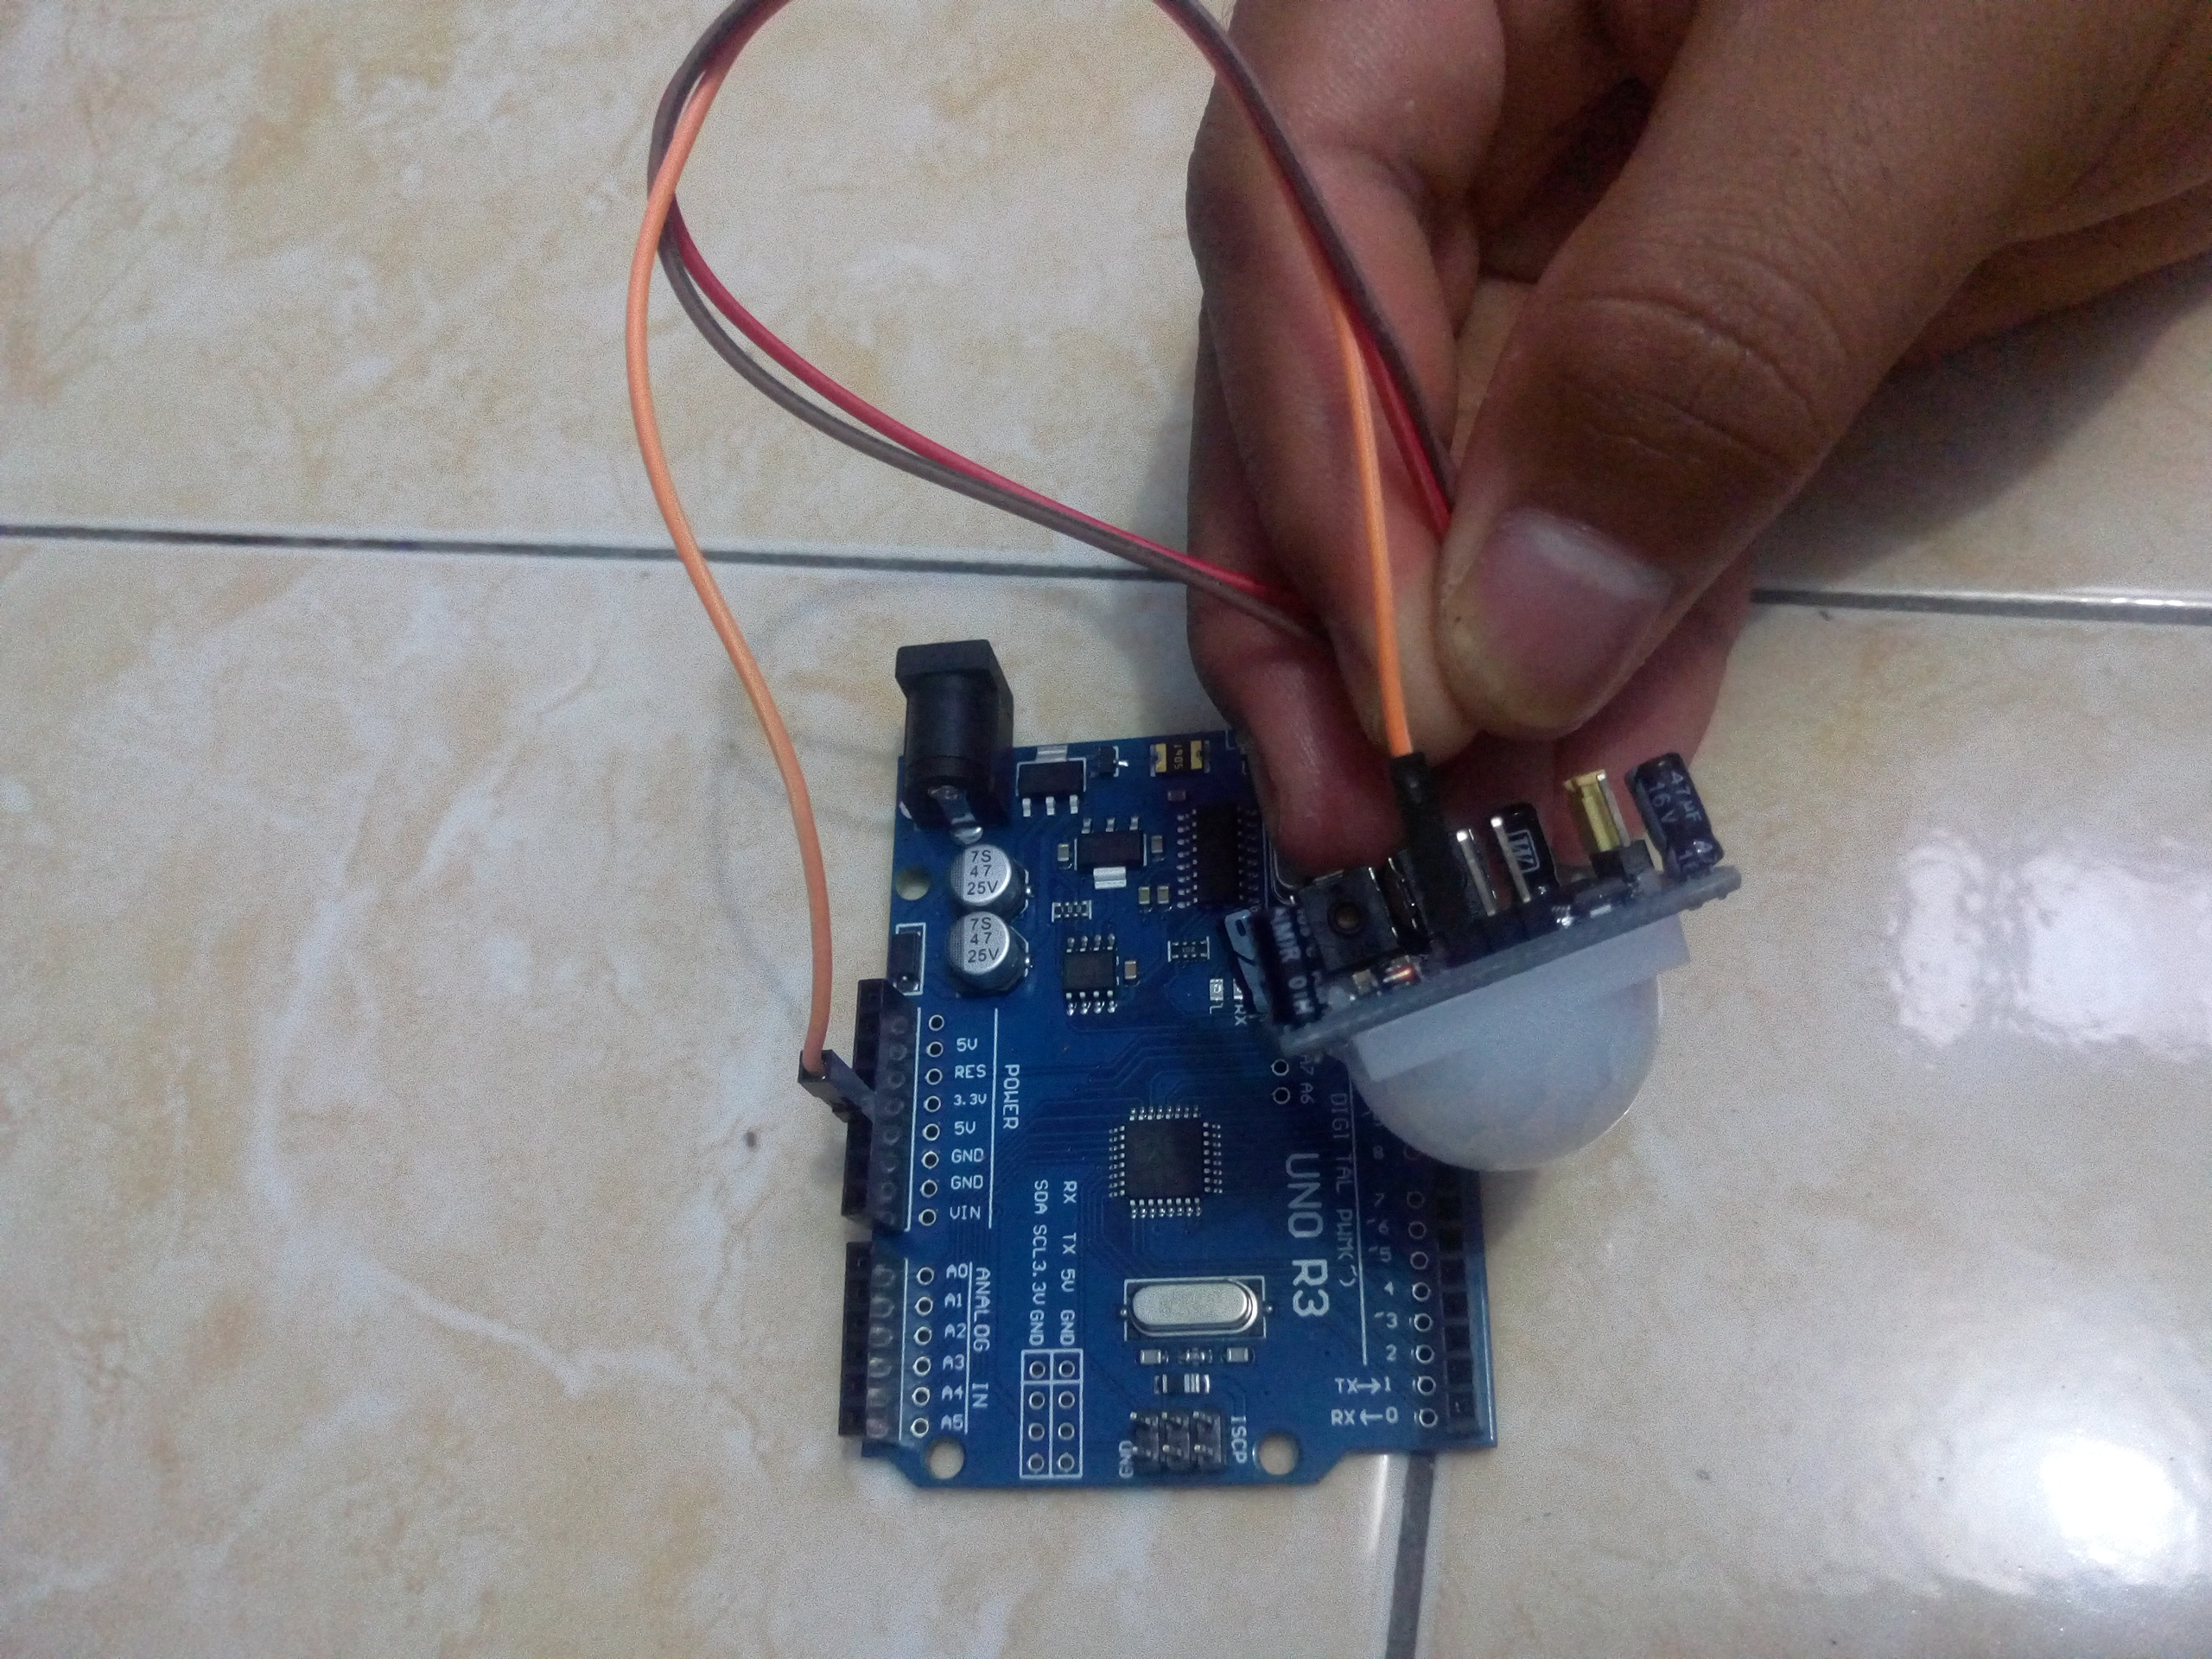
\includegraphics[width=1\textwidth]{figures/kabelvcc.JPG}}
\caption{gambar kabelvcc.}
\label{carakoneksikabelvcc}
\end{figure}

b. Gabungkan kabel jumper male to female berwarna merah dari OUPUT sensor pir ke pin A5 arduino(gambar \ref{ckkabeloutput})

\begin{figure} [ht]
\centerline{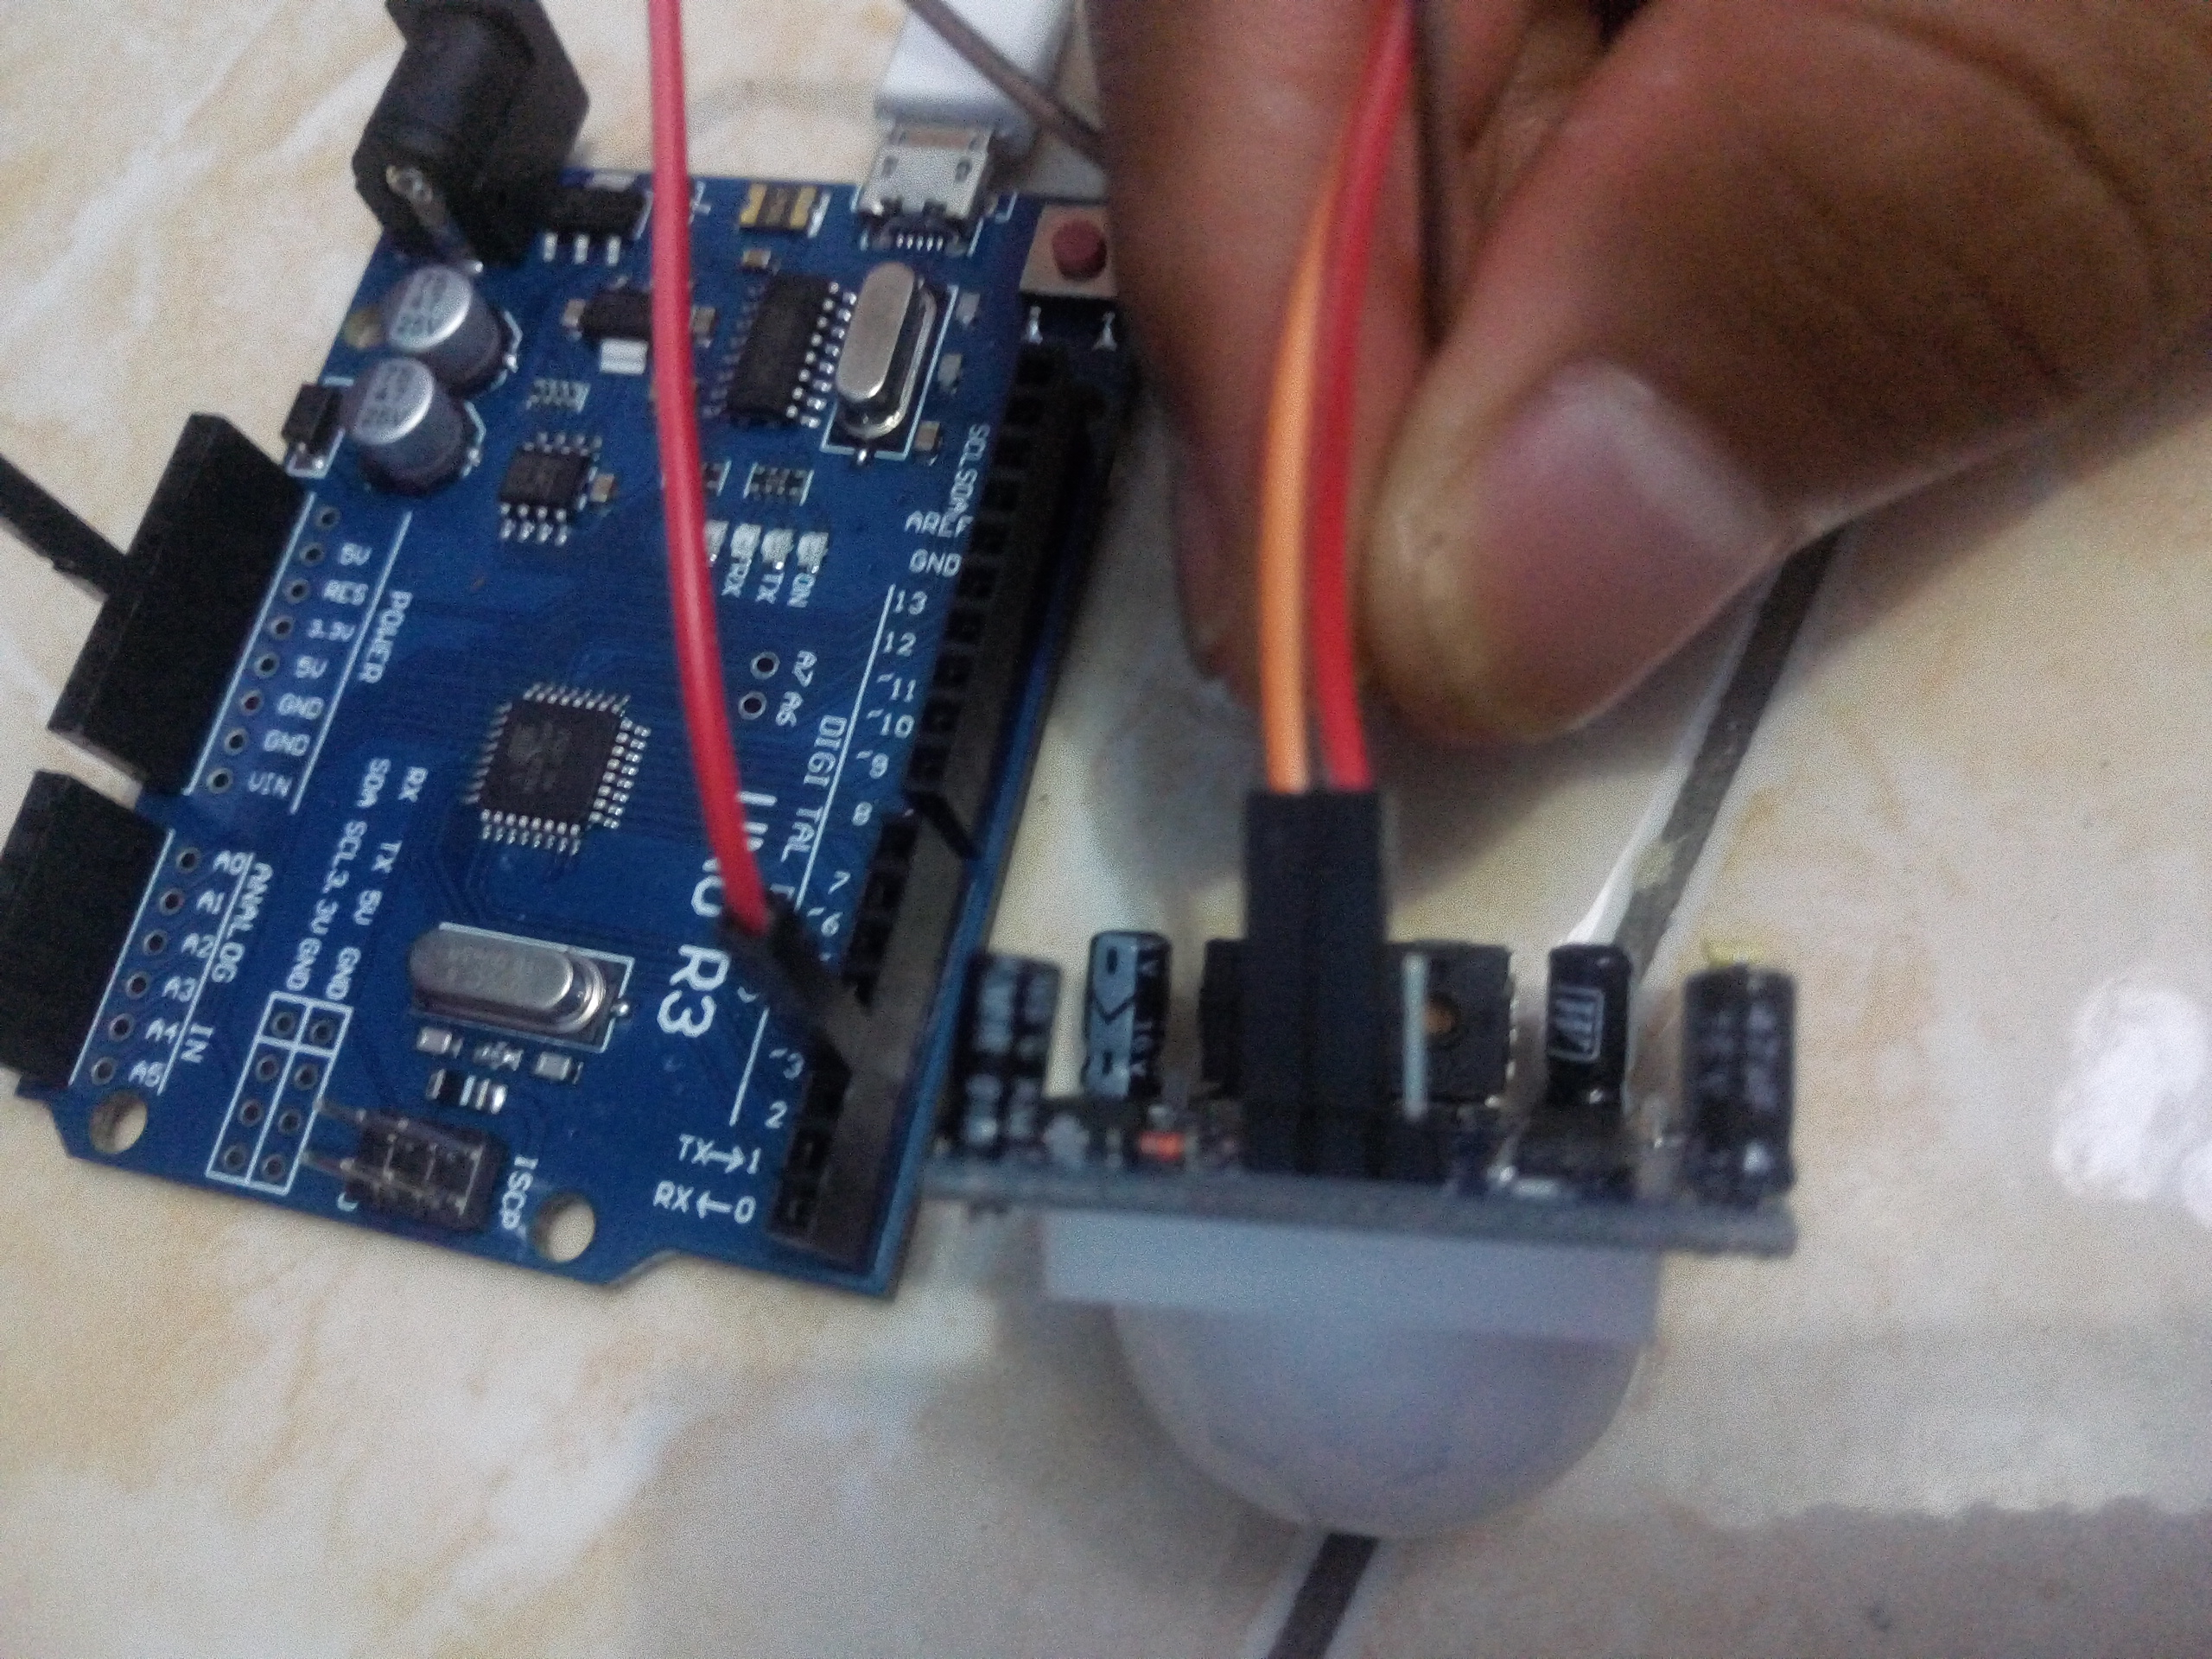
\includegraphics[width=1\textwidth]{figures/kabeloutput.JPG}}
\caption{gambar kabeloutput.}
\label{ckkabeloutput}
\end{figure}

c. Gabungkan kabel jumper male to female berwarna coklate dari GND sensor pir ke GND arduino(gambar \ref{ckkabelgnd})

\begin{figure} [ht]
\centerline{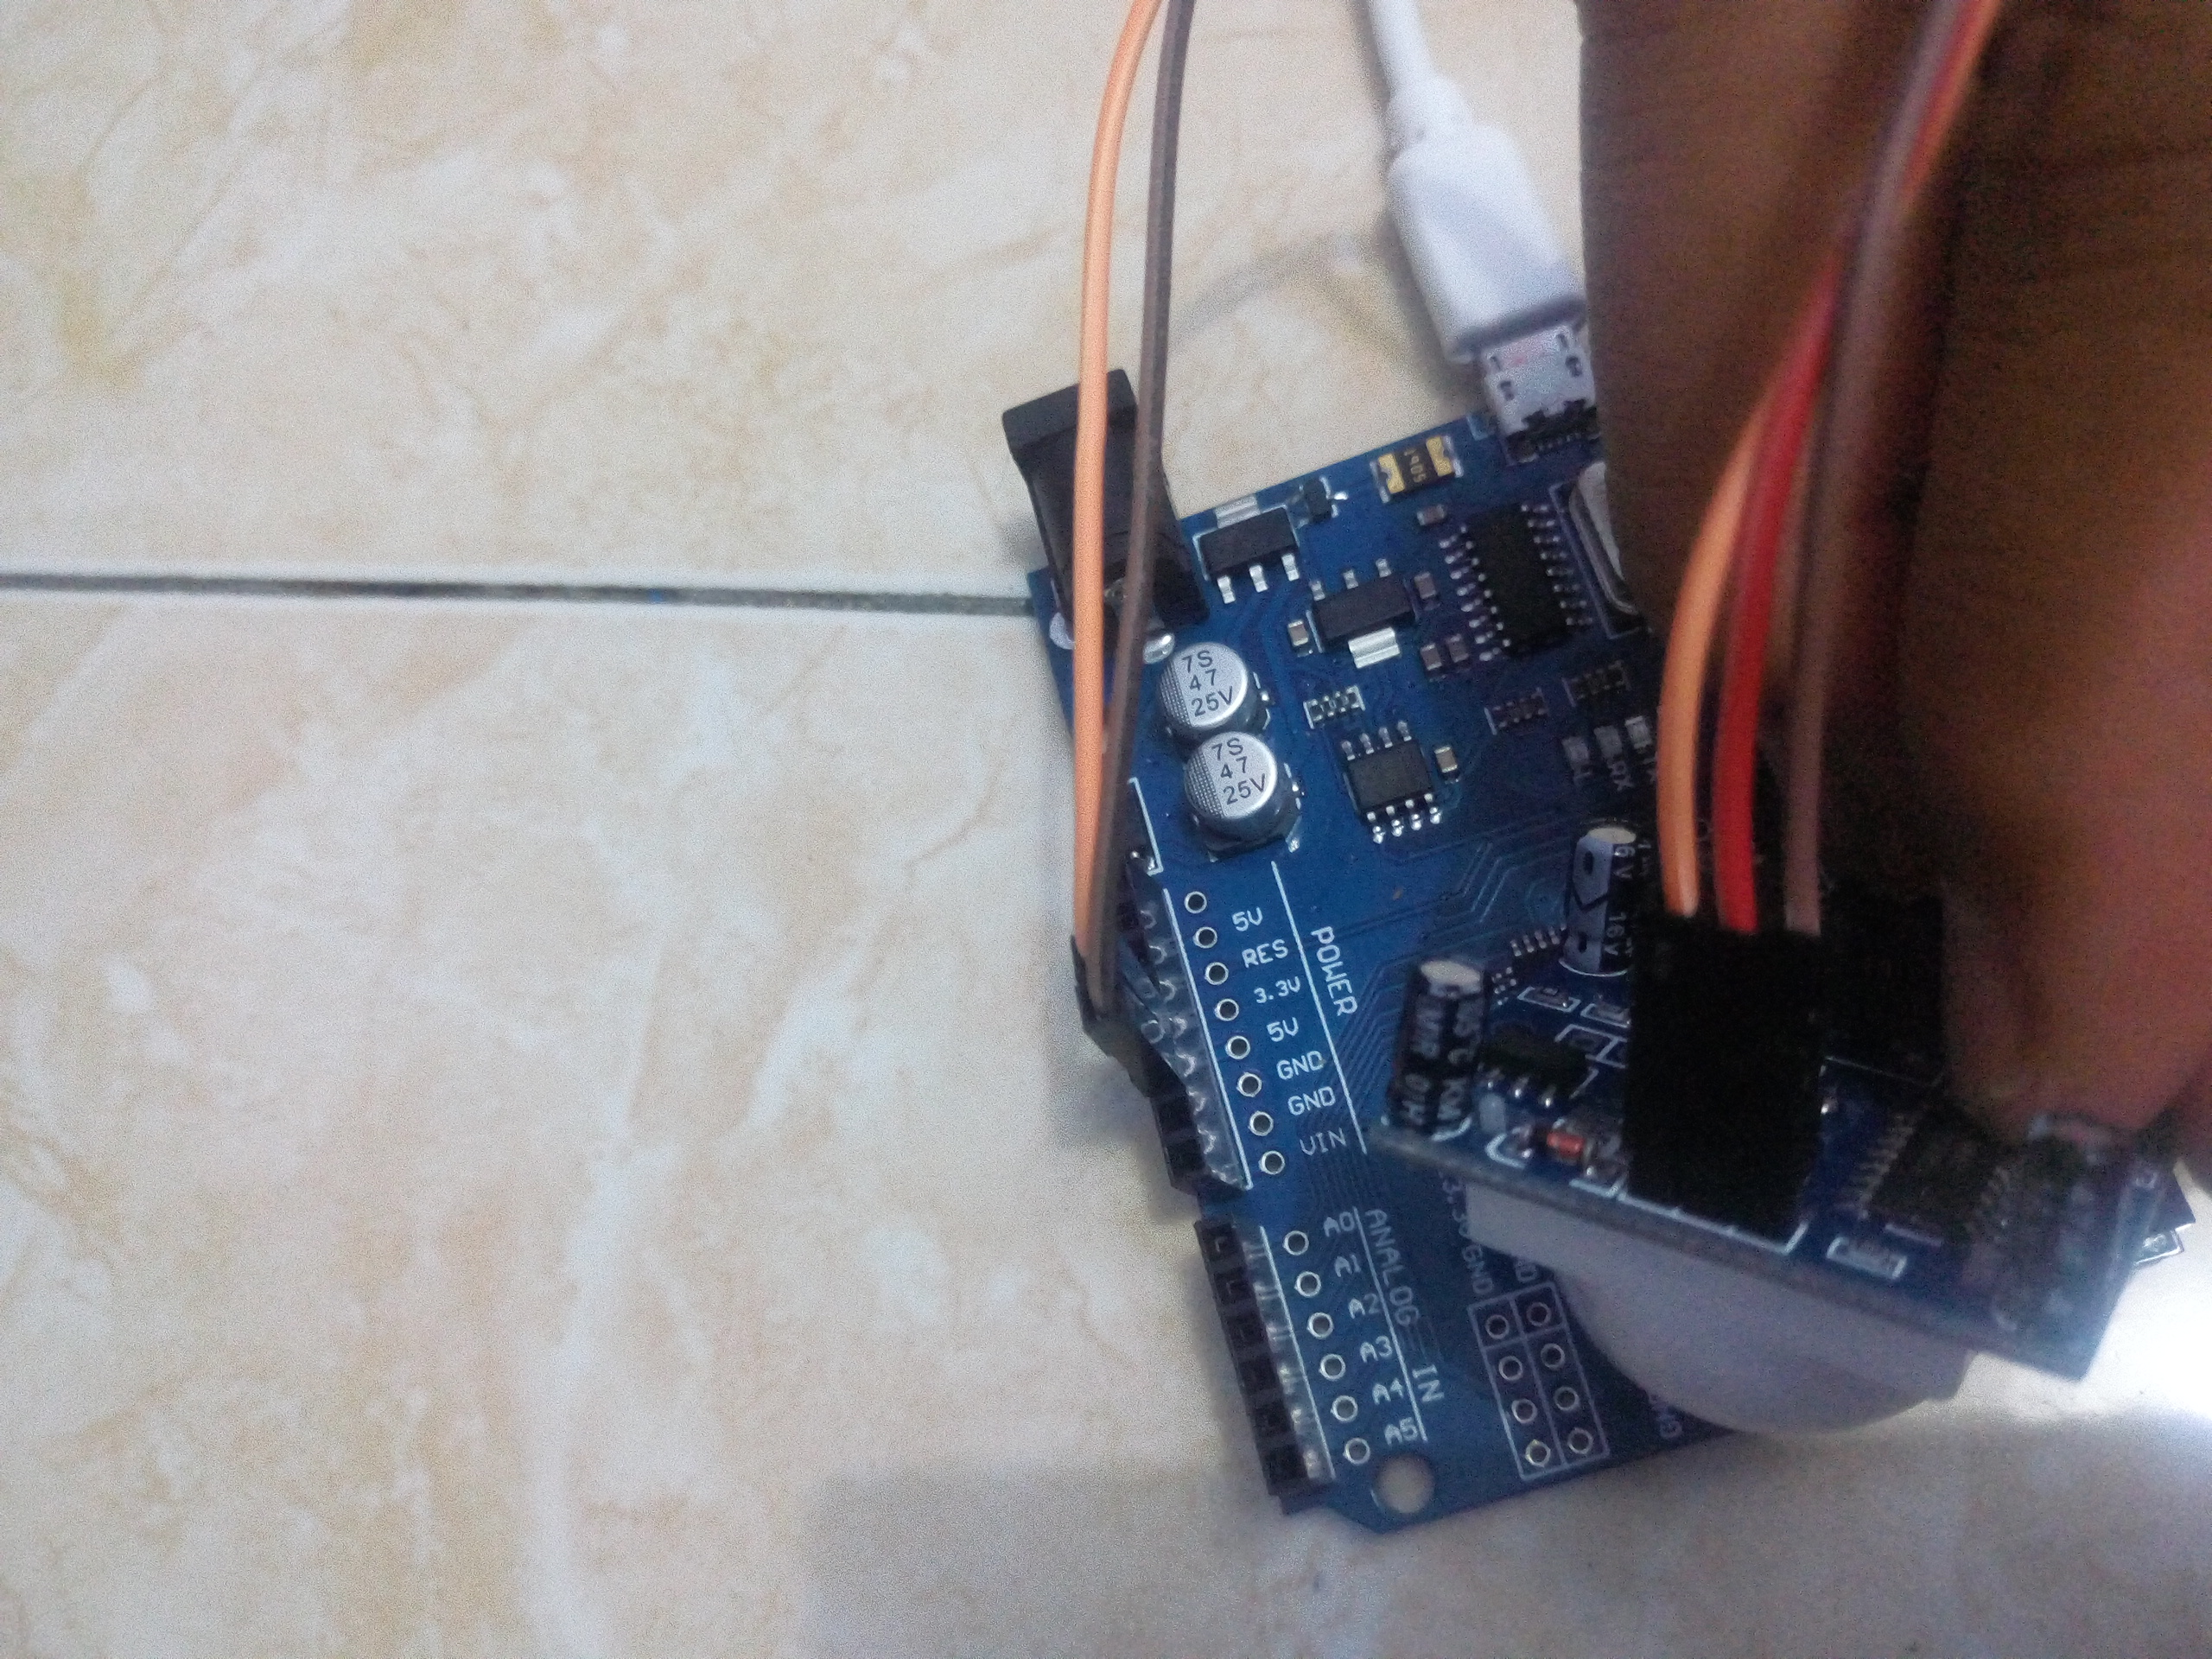
\includegraphics[width=1\textwidth]{figures/kabelgnd.JPG}}
\caption{gambar kabelgnd.}
\label{ckkabelgnd}
\end{figure}

d. Pasang lampu led berwarna biru ke pin 13 arduino. lihat di gambar \ref{ckled}.

\begin{figure} [ht]
\centerline{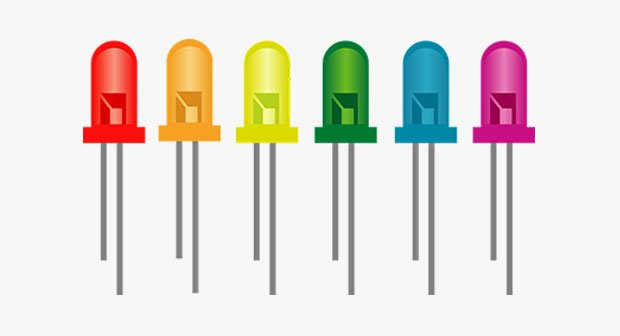
\includegraphics[width=1\textwidth]{figures/led.JPG}}
\caption{gambar led.}
\label{ckled}
\end{figure}

e. Pasang kabel USB dari arduino ke PC seperti pada gambar \ref{ckkabelusb}.

\begin{figure} [ht]
\centerline{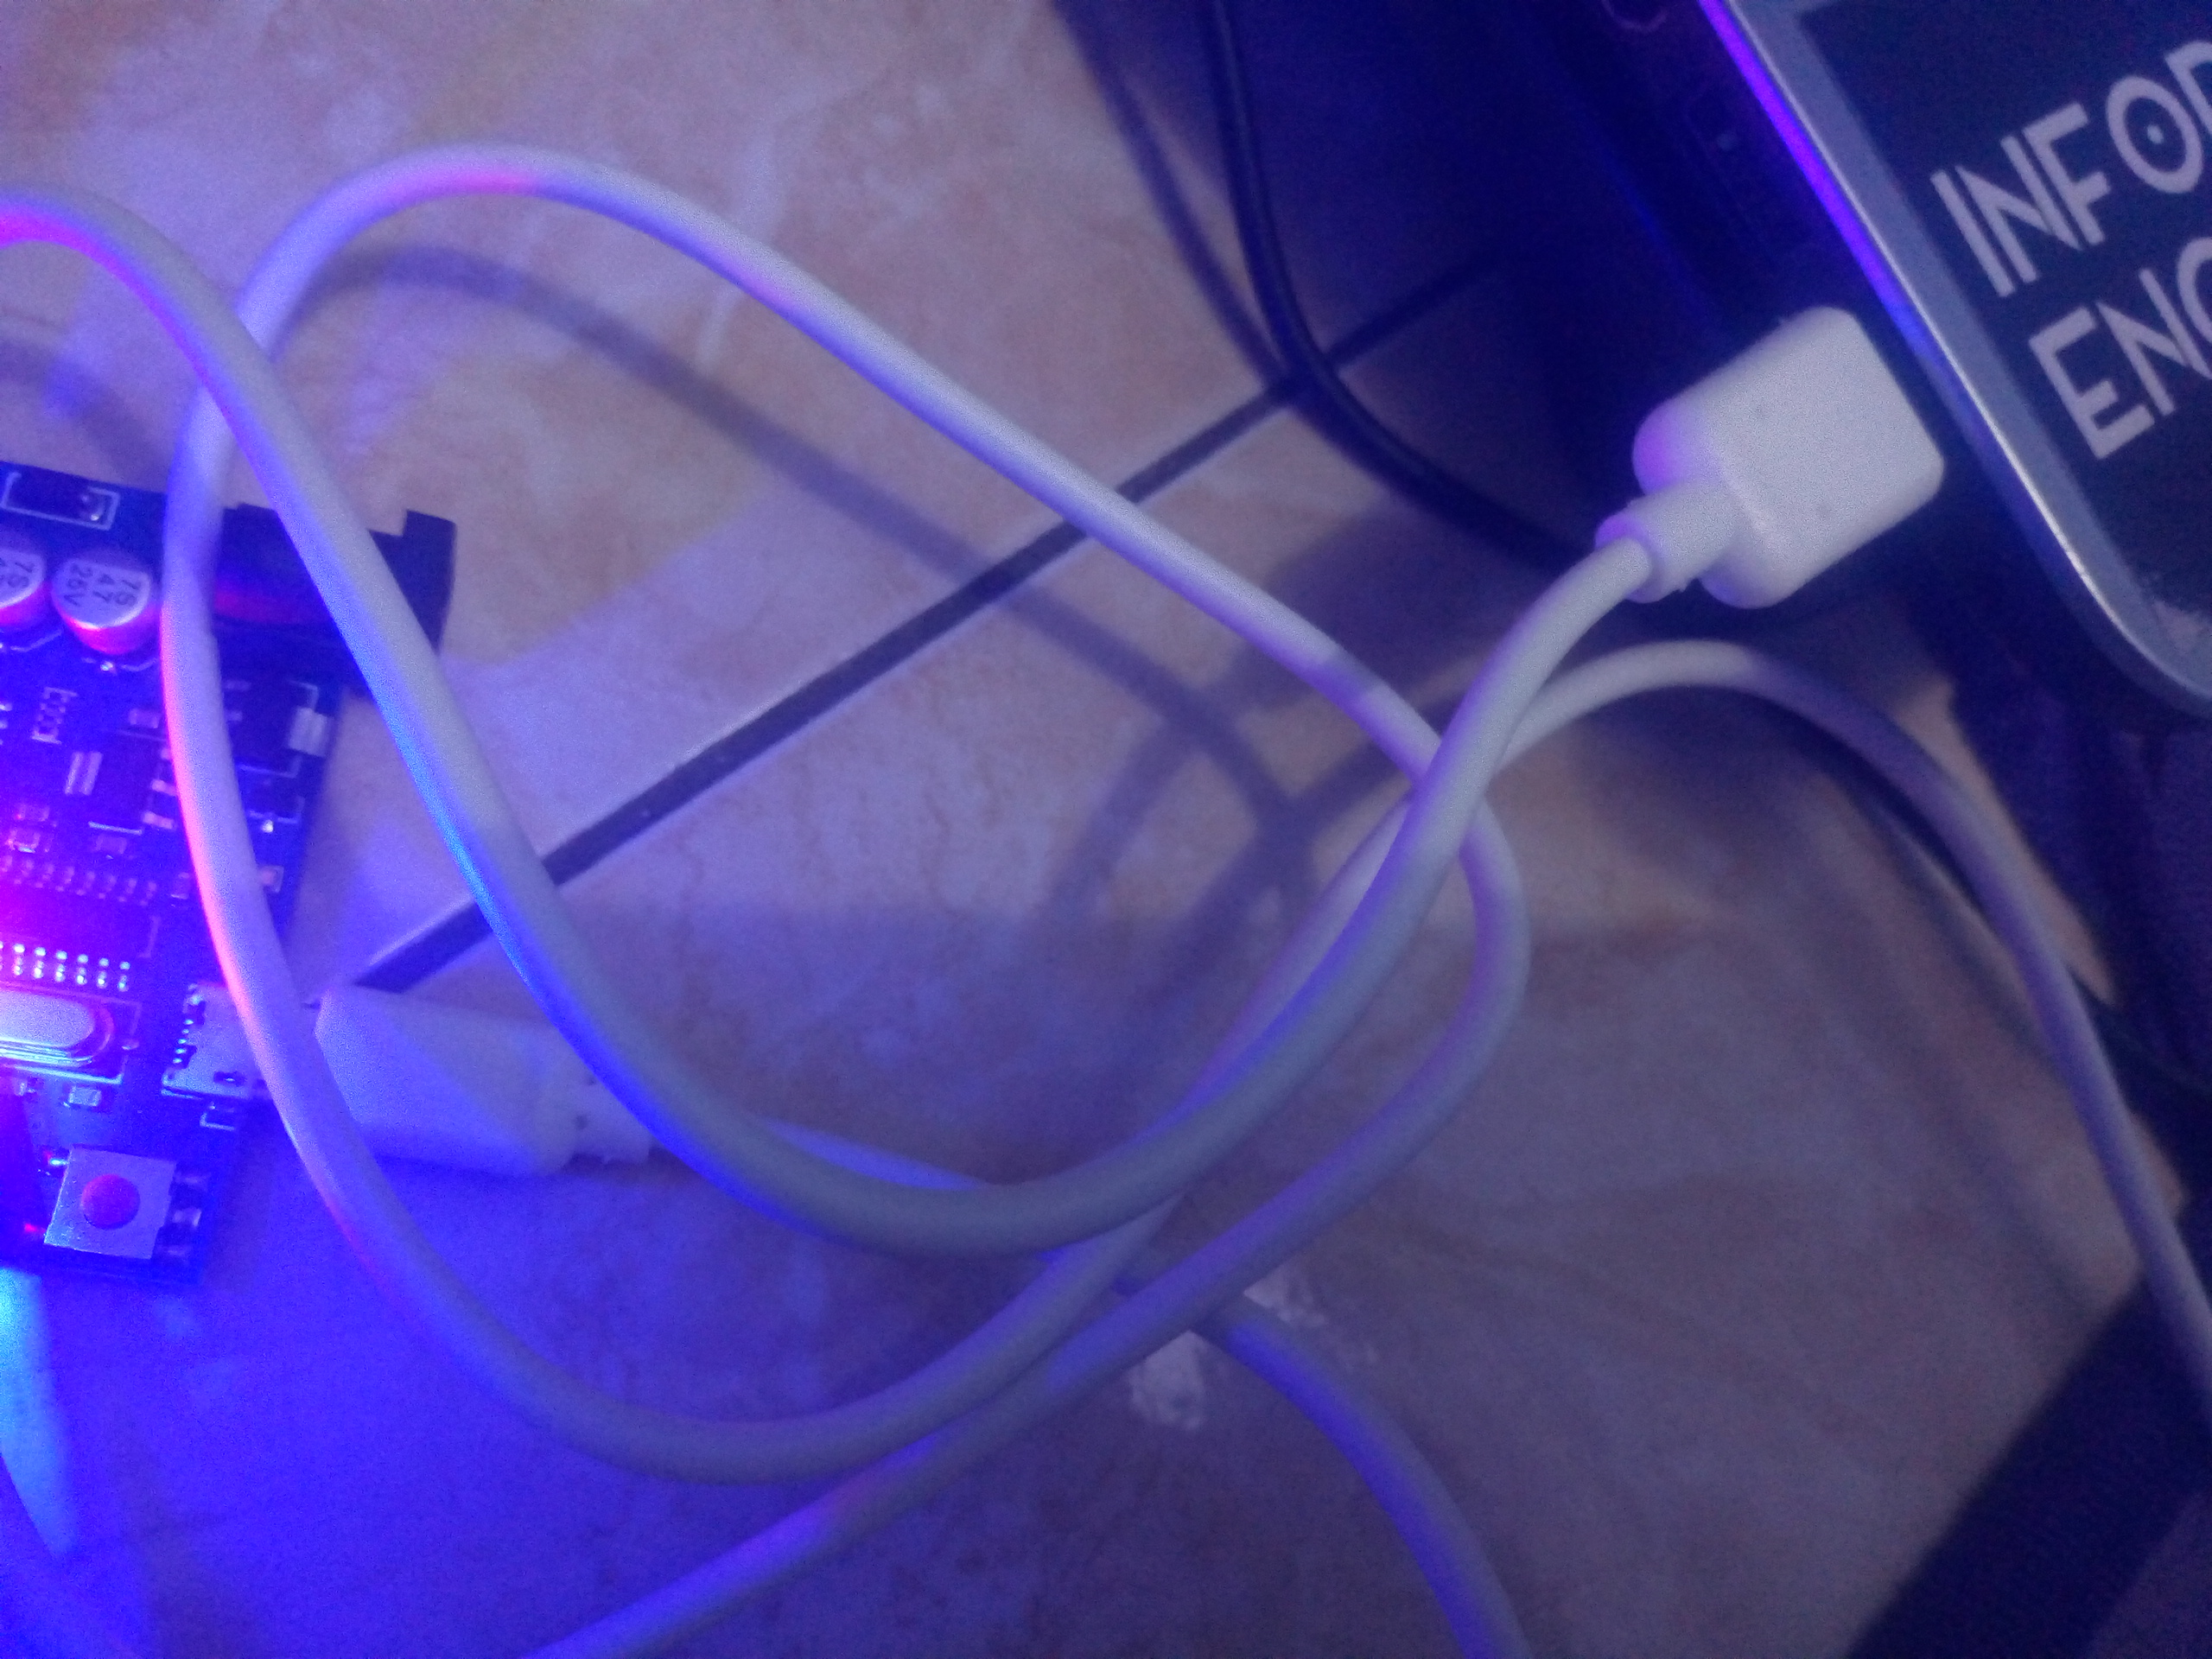
\includegraphics[width=1\textwidth]{figures/kabelusb.JPG}}
\caption{gambar kabelusb.}
\label{ckkabelusb}
\end{figure}

f. Buat Codingan Sensor Pir seperti gambar \ref{coding}.

\begin{figure} [ht]
\centerline{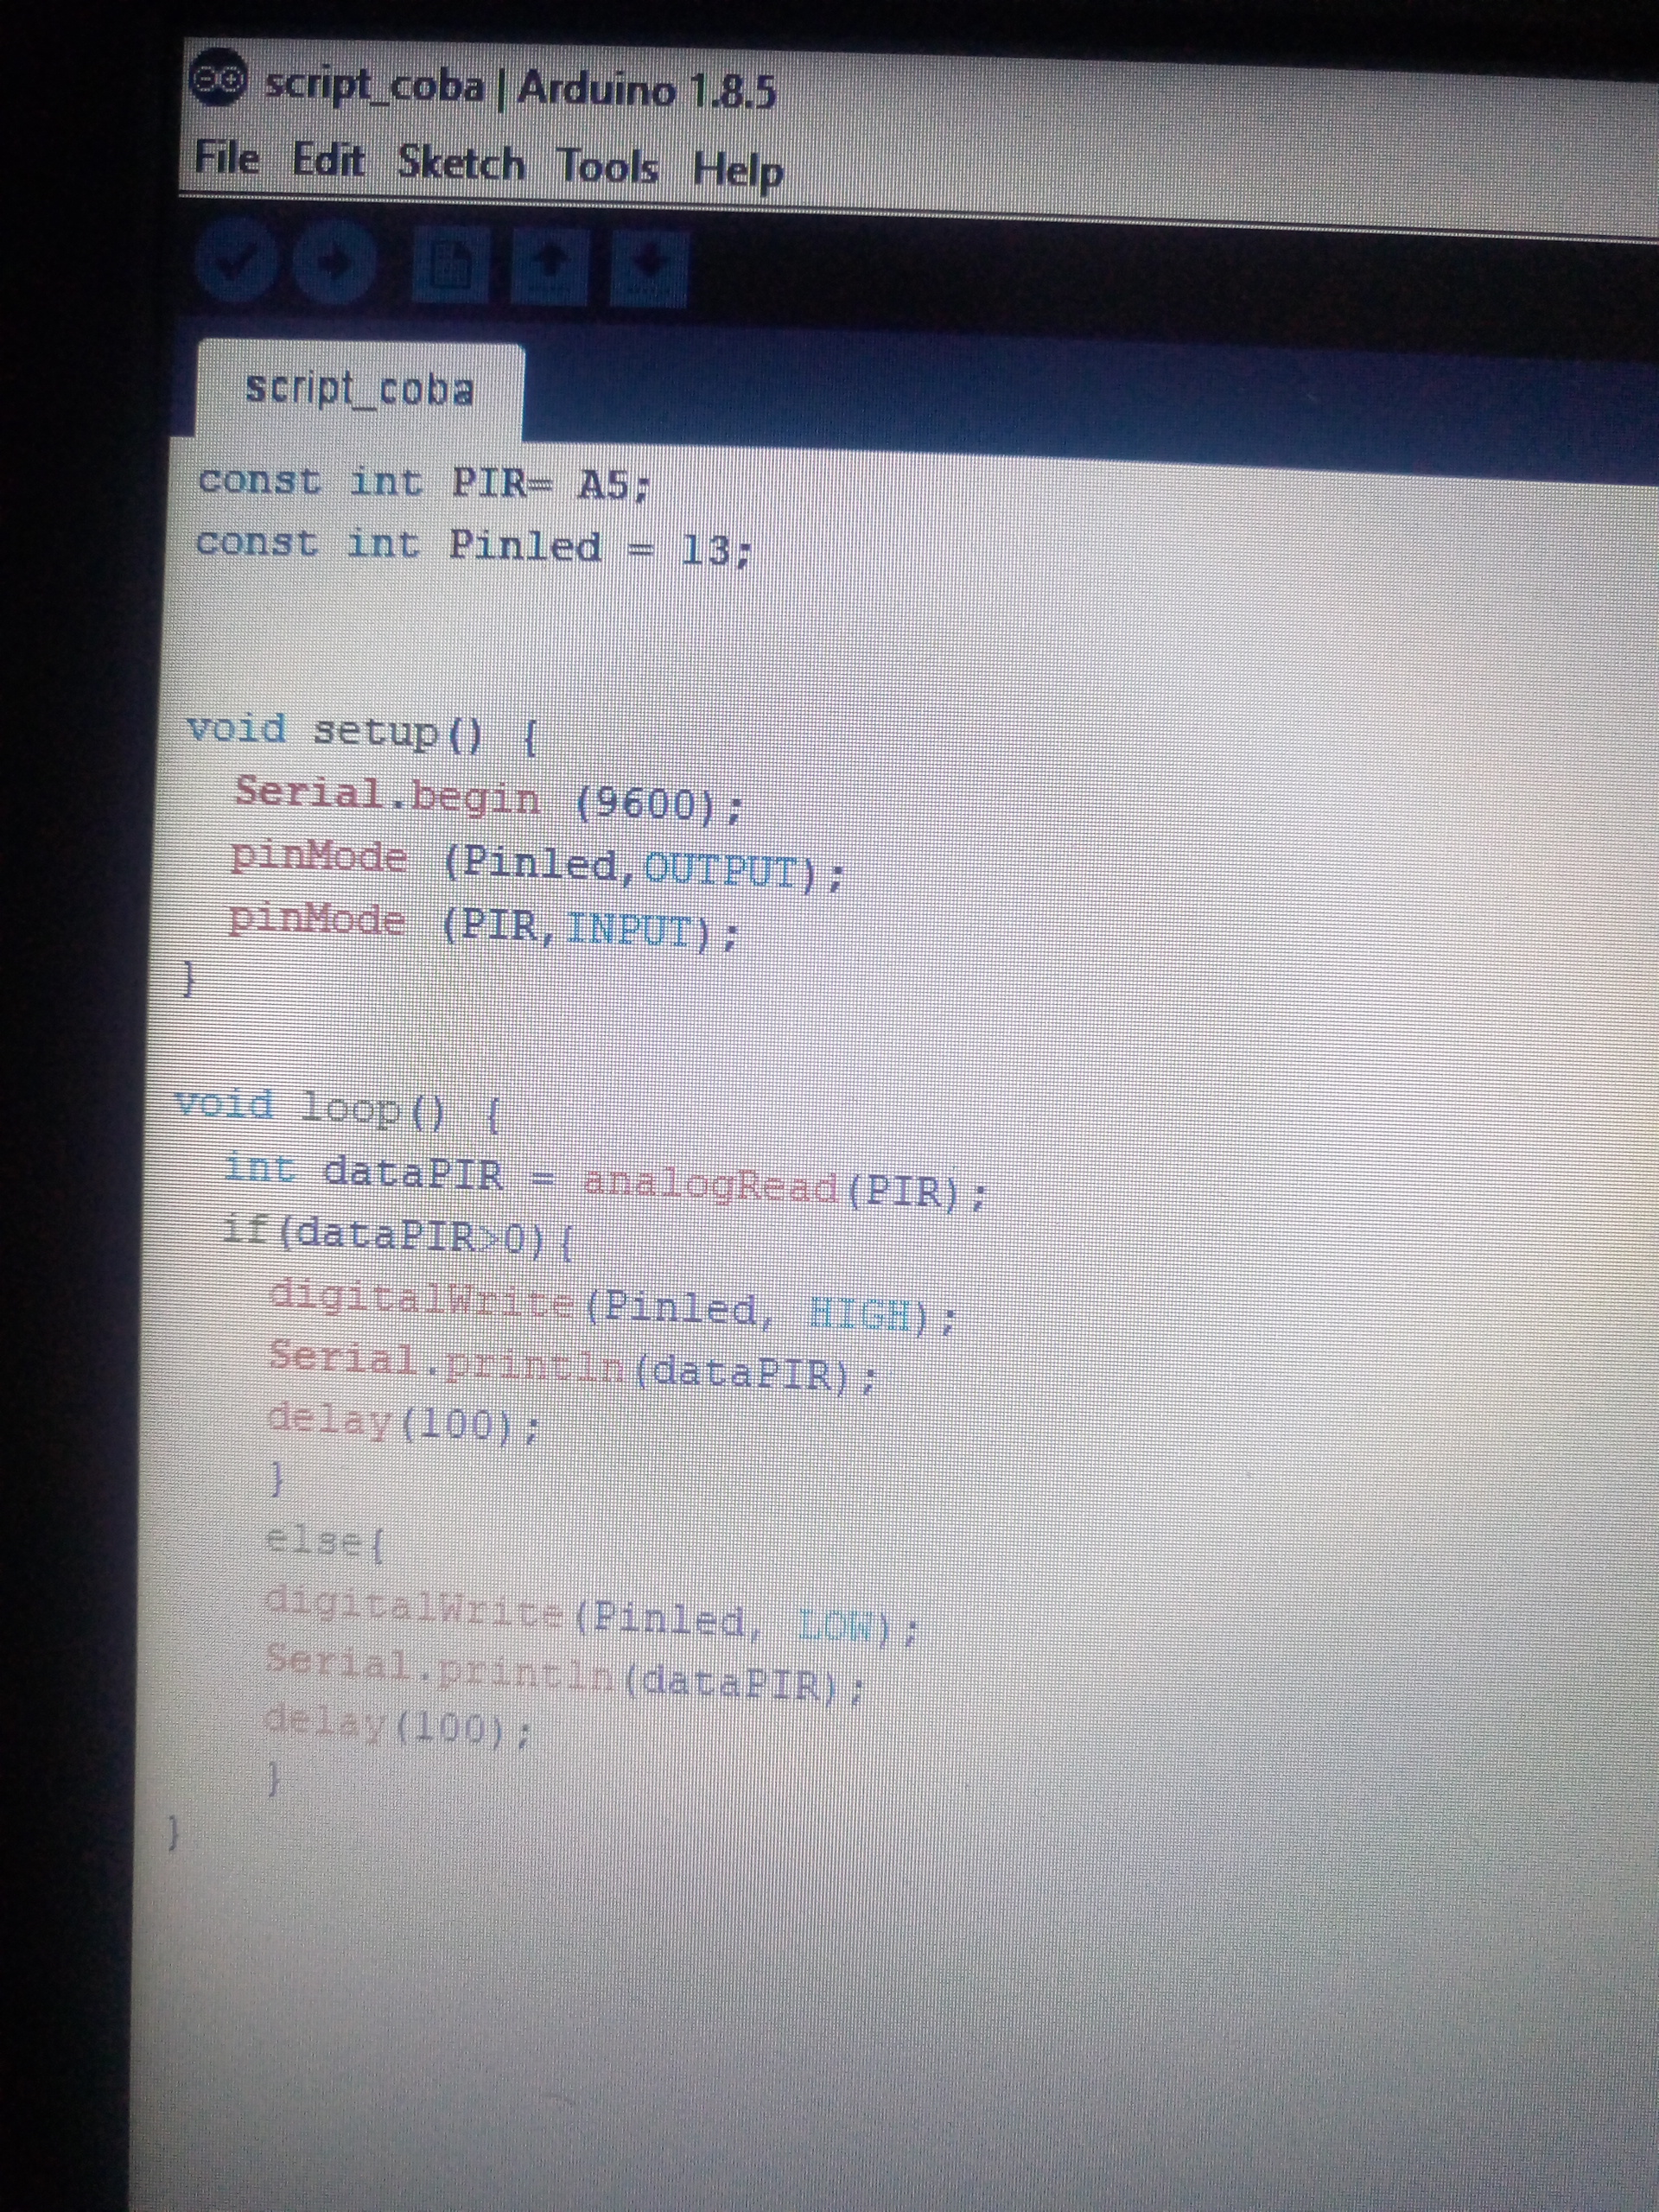
\includegraphics[width=1\textwidth]{figures/coding.JPG}}
\caption{gambar coding.}
\label{coding}
\end{figure}

\subsection {Kegunaan sensor PIR}
Sensor ini bekerja dengan cara membaca gerakan pada jarak tertentu, jarak ini yang sangat mempengaruhi sensor semakin dekat jarak benda bergerak maka semakin gampang pula sensor membaca gerakan.
Biasanya sensor ini digunakan pada pintu mall otomatis.
